\documentclass{beamer}
\usepackage[english,activeacute]{babel}
\usepackage[utf8]{inputenc}
\usepackage{listings}
\usepackage{color}
\usepackage{tikz}

\definecolor{red}{RGB}{255,0,0}
\definecolor{green}{RGB}{0,255,0} 
\definecolor{blue}{RGB}{0,0,255} 
\definecolor{oran}{RGB}{255,93,0} 

\newcommand{\blue}{\textcolor{blue}}
\newcommand{\red}{\textcolor{red}}
\newcommand{\green}{\textcolor{green}}
\newcommand{\oran}{\textcolor{oran}}
\definecolor{gray97}{gray}{.97}
\definecolor{gray75}{gray}{.75}
\definecolor{gray45}{gray}{.45}

\renewcommand\mathfamilydefault{\rmdefault}

\usetheme[pageofpages=of,
          alternativetitlepage=true,
          titlepagelogo=img/aei,
          watermark=,
          watermarkheight=50px,
          watermarkheightmult=1,
          ]{Torino}

\lstset{ frame=Ltb,
     framerule=0pt,
     aboveskip=0.5cm,
     framextopmargin=3pt,
     framexbottommargin=3pt,
     framexleftmargin=0.4cm,
     framesep=0pt,
     rulesep=.4pt,
     backgroundcolor=\color{gray97},
     rulesepcolor=\color{black},
     %
     stringstyle=\ttfamily,
     showstringspaces = false,
     basicstyle=\tiny\ttfamily,
     %commentstyle=\color{gray45},
     %keywordstyle=\bfseries,
     %
     numbers=left,
     numbersep=13pt,
     numberstyle=\tiny,
     numberfirstline = false,
     breaklines=true,
     emph = {[1]\_\_device\_\_,\_\_global\_\_,\_\_syncthreads,pthread\_create,pthread\_join,pragma,omp,parallel,private, threadIdx, blockDim, blockIdx,cudaThreadSynchronize},
     emphstyle={[1]\color{blue}},
   }

% minimizar fragmentado de listados
\lstnewenvironment{listing}[1][]
   {\lstset{#1}\pagebreak[0]}{\pagebreak[0]}

\lstdefinestyle{consola}
   {basicstyle=\scriptsize\bf\ttfamily,
    backgroundcolor=\color{gray75},
   }
\lstdefinestyle{C}
   {language=C,
   }



\usecolortheme{nouvelle}
\vspace{-0.5cm}
\author[Cristián Maureira]
       {\large Cristián Maureira\\
        \small \textcolor{gray}{Computer Science Master Student, UTFSM}}
\title[GraviDy]
      {\huge GraviDy}
\subtitle{\Large A modular direct N-body GPU integrator.}
\institute[AEI]
          {Albert Einstein Institute}

\begin{document}

% First slide
\begin{frame}[t,plain]
    \titlepage
\end{frame}

\section{Introduction}

\begin{frame}
    \frametitle{Agenda}
    \begin{itemize}
        \item GPU Computing.
        \item The GraviDy project.
        \item Future work and discussion.
    \end{itemize}
\end{frame}


%
%
%\begin{frame}
%    \frametitle{Introduction}
%    \framesubtitle{The initial idea}
%    \begin{enumerate}
%        \item N-body introduction?
%        \item The problems related to the galactic center,
%              or planetary systems...?
%        \item The widely know N-body integrators have problems
%              with the Energy conservation...?
%    \end{enumerate}
%\end{frame}
%
%\begin{frame}
%    \frametitle{Introduction}
%    \framesubtitle{Why write a new integrator?}
%    \begin{itemize}
%            \item Previous work:
%            \begin{itemize}
%                \item Aarseth integrators (NBODY0, NBODY1, ..., NBODY7)
%                \item Gravity Pipe (GRAPE).
%            \end{itemize}
%            \item GPU is replacing the CPU to perform scientific calculations.
%                 \emph(``General Purpose computing on GPUs'' - \url{http://gpgpu.org})
%            \item ...another reason.
%    \end{itemize}
%\end{frame}
%
%\begin{frame}
%    \frametitle{Introduction}
%    \framesubtitle{Parallel computing background}
%    \begin{description}
%        \item[Task parallelism]
%            Each processor perform a self task.
%        \item[Data parallelism]
%            Each processor perform the same task, but on its own data set.
%    \end{description}
%\end{frame}
%
%\begin{frame}
%    \frametitle{Introduction}
%    \framesubtitle{Parallel computing background}
%    \begin{description}
%        \item[Performance]
%                Capacity of perform individual instructions in a certain time.
%        \item[Throughput]
%                Capacity of perform a whole task in a certain time.
%        \item[Latency]
%                Measure of time delay experienced in a system.
%        \item[Granularity]
%                Broke down a system into small parts.(Coarse and Fine)
%    \end{description}
%\end{frame}
%

\begin{frame}
    \frametitle{GPU Computing}
    \framesubtitle{Introduction}
    \begin{itemize}
        \item At the beggining, programming in GPU was really difficult.
        \item Now, there are a lot of languages, applications, libraries, etc
            who really help to enter in the GPU Computing world.
        \begin{itemize}
            \item OpenCL, CUDA.
            \item MATLAB.
            \item CUBLAS, CUSP, Thrust, etc.
        \end{itemize}
    \end{itemize}
\end{frame}

\begin{frame}
    \frametitle{GPU Computing}
    \framesubtitle{Architecture}
    \begin{figure}
        \centering
        \label{fig:architecture}
        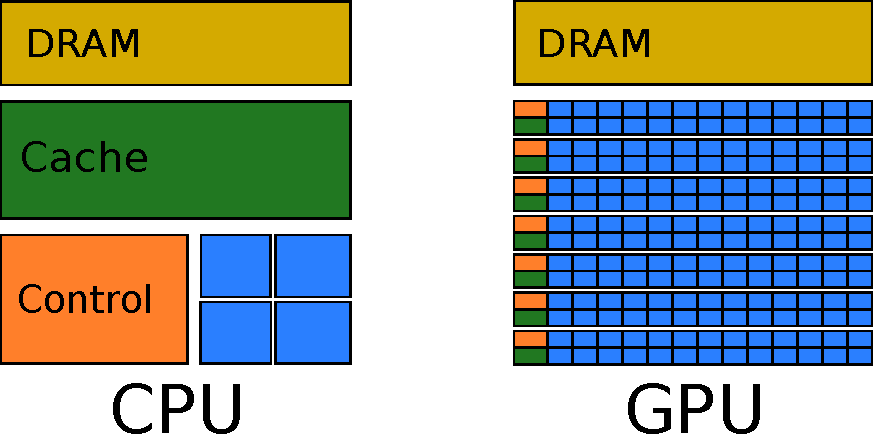
\includegraphics[width=0.8\textwidth]{img/architecture.pdf}
        \caption{CPU and GPU simplistic architecture model}
    \end{figure}
\end{frame}

\begin{frame}
    \frametitle{GPU Computing}
    \framesubtitle{Differences between CPU and GPU}
    \begin{itemize}
        \item Goals and design
        \begin{itemize}
            \item The CPU was designed to have a good performances with parallel and non-parallel
                  scenarios.
            \item The GPU was dessigned to do highly parallel work.
        \end{itemize}
        \item The CPU minimize \blue{latency} experienced by 1 thread (big on-chip caches).
        \item The GPU maximize \blue{throughput} of all threads.
    \end{itemize}
\end{frame}

\begin{frame}
    \frametitle{CUDA}
    \framesubtitle{Introduction}
    \begin{itemize}
        \item 
    \end{itemize}
\end{frame}

\begin{frame}
    \frametitle{CUDA}
    \framesubtitle{Program structure}
    \begin{figure}
        \centering
        \label{fig:cuda-structure}
        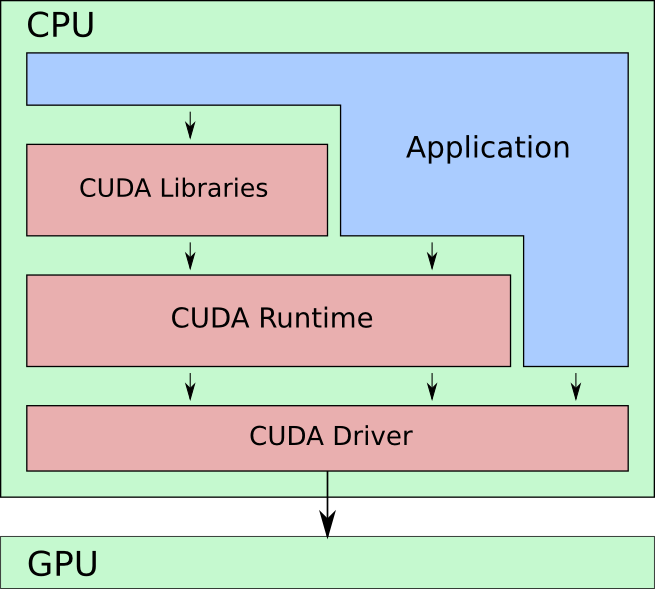
\includegraphics[width=0.5\textwidth]{img/cuda-structure}
        \caption{Program structure}
    \end{figure}
\end{frame}

\begin{frame}
    \frametitle{CUDA}
    \framesubtitle{Program structure - Example}

    ...
\end{frame}



\begin{frame}
    \frametitle{CUDA}
    \framesubtitle{Threads and blocks}
    \begin{itemize}
        \item 
    \end{itemize}
\end{frame}

\begin{frame}
    \frametitle{CUDA}
    \framesubtitle{Memories}
    \begin{figure}
        \centering
        \label{fig:cuda-memories}
        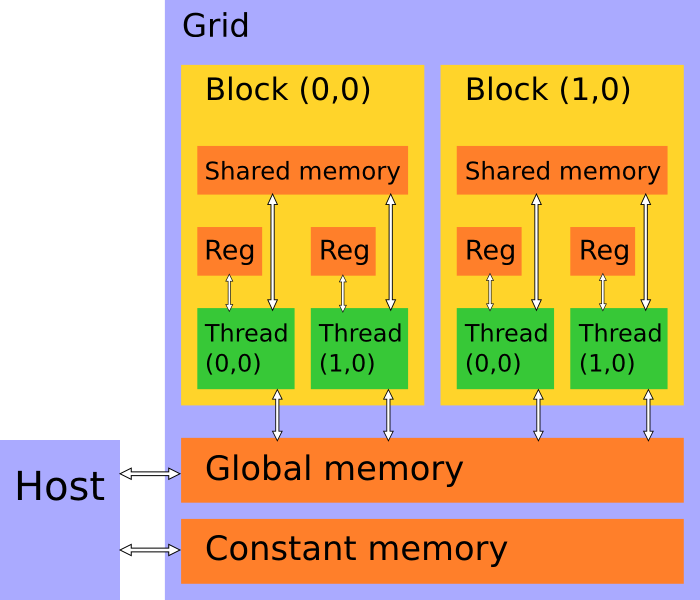
\includegraphics[width=0.5\textwidth]{img/cuda-memories}
        \caption{GPU Memories}
    \end{figure}
\end{frame}

\begin{frame}[fragile]
    \frametitle{CUDA}
    \framesubtitle{Memories}
    \begin{table}
    \centering
    \label{tab:memories-penalty}
    \scriptsize
    \begin{tabular}{l|r|r|r|r}
        \textbf{Declaration}  & \textbf{Memory}   & \textbf{Scope}  & \textbf{Lifetime}    & \textbf{Penalization} \\
        \texttt{int var;}                      & Register & Thread & Thread      & 1x \\
        \texttt{int a\_var[10];}            & Local    & Thread & Thread      & 100x \\
        \texttt{\_\_shared\_\_ int sh\_var;}    & Shared   & Block  & Block       & 1x \\
        \texttt{\_\_device\_\_ int gl\_var;}    & Global   & Grid   & Application & 100x \\
        \texttt{\_\_constant\_\_ int ct\_var;}& Constant & Grid   & Application & 1x 
    \end{tabular}
    \label{CUDA Memories}
    \end{table}
\end{frame}

\begin{frame}
    \frametitle{CUDA}
    \framesubtitle{Memories - Example}

    ...
\end{frame}

\begin{frame}
    \frametitle{CUDA}
    \framesubtitle{Programming strategy}
    \begin{figure}
        \centering
        \label{fig:cuda-strategy}
        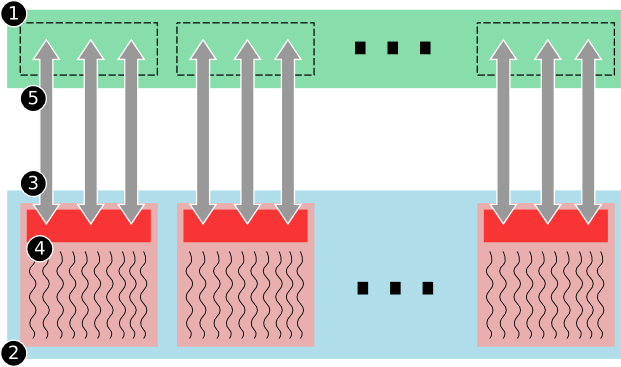
\includegraphics[width=0.6\textwidth]{img/cuda-strategy}
        \caption{GPU programming strategy}
    \end{figure}
\end{frame}

\begin{frame}
    \frametitle{CUDA}
    \framesubtitle{Programming strategy - Example}
    ...
\end{frame}

\begin{frame}
    \frametitle{GraviDy}
    \framesubtitle{Introduction}
    \begin{center}
        A semi-keplerian N-body integrator...?
    \end{center}
\end{frame}

\begin{frame}
    \frametitle{GraviDy}
    \framesubtitle{Features}
    \begin{itemize}
        \item Based on a 4th order Hermite integrator.
        \item Using block timesteps.
        \item Add keplerian treatment to work with the massive central object.
              (Loeckmann dissertation reference).
    \end{itemize}
\end{frame}

\begin{frame}
    \frametitle{GraviDy}
    \framesubtitle{Code}
    \begin{itemize}
        \item Written in C++ and CUDA.
        \item Modular developing.
        \item Aims to take the BHINT main idea.
    \end{itemize}
\end{frame}

\begin{frame}
    \frametitle{GraviDy}
    \framesubtitle{Predictor-Corrector procedure}
    \begin{enumerate}
        \item Initial $a$ and $a^{(1)}$ calculation.
        \item Initial block timesteps calculation.
        \item Select particles to move.
        \begin{enumerate}
            \item Calculate the predicted position and velocity.
            \item Calculate the $a$, $a^{(1)}$, $a^{(2)}$ and $a^{(3)}$.
            \item Apply the correction to the position and velocity.
            \item Update timesteps.
        \end{enumerate}
    \end{enumerate}
\end{frame}

\begin{frame}
    \frametitle{GraviDy}
    \framesubtitle{BHINT approach}
    \begin{eqnarray}
        \boldsymbol{a}_{i} =   \underbrace{ - G m_{0}
                                          \dfrac{\boldsymbol{r}_{i}}{r_{i}^{3}}
                                          }_{unperturbed\ motion}
                             - \underbrace{ \sum\limits_{\substack{j=1\\j\neq i}}^{N-1}
                                            G m_{j} \dfrac{\boldsymbol{r}_{ij}}{r_{ij}^{3}}
                                          }_{perturbing\ force}
    \end{eqnarray}
\end{frame}

\begin{frame}
    \frametitle{GraviDy}
    \framesubtitle{Kepler's correction}
    \begin{enumerate}
        \item This is applied to the \blue{Predicted} step.
        \item The normal Hermite formula is:
        \begin{eqnarray}
            \boldsymbol{r}_{pred} =    \boldsymbol{      r}_{i}              +
                                       \boldsymbol{      v}_{i} \Delta t     +
                         \dfrac{1}{2!} \boldsymbol{      a}_{i} \Delta t^{2} +
                         \dfrac{1}{3!} \boldsymbol{\dot{a}}_{i} \Delta t^{3}
        \end{eqnarray}
        \item With the Kepler's correction:
        \begin{eqnarray}
            \boldsymbol{r}_{pred} =    \blue{\boldsymbol{      r}_{k,pred}}         +
                                             \boldsymbol{      v}_{i} \Delta t     +
                         \dfrac{1}{2!}       \boldsymbol{      a}_{i} \Delta t^{2} +
                         \dfrac{1}{3!}       \boldsymbol{\dot{a}}_{i} \Delta t^{3}
        \end{eqnarray}
        \item where $\boldsymbol{r}_{k}$ and its derivates 
            are obtained from the unperturbed motion along a Keplerian orbit,
        \begin{eqnarray}
            \blue{\boldsymbol{r}_{k,pred}} =  \boldsymbol{      r}_{k}              +
                                       \boldsymbol{      v}_{k} \Delta t     +
                         \dfrac{1}{2!} \boldsymbol{      a}_{k} \Delta t^{2} +
                         \dfrac{1}{3!} \boldsymbol{\dot{a}}_{k} \Delta t^{3}
        \end{eqnarray}

    \end{enumerate}
\end{frame}

\begin{frame}
    \frametitle{Preliminar results}
    \begin{figure}
        \centering
        \label{fig:init-time}
        %\includegraphics[width=0.8\textwidth]{img/result-init_accjerk}
        \caption{Initial $a$ and $\dot{a}$ calculation}
    \end{figure}
\end{frame}

\begin{frame}
    \frametitle{Preliminar results}
    \begin{figure}
        \centering
        \label{fig:init-time}
        %\includegraphics[width=0.8\textwidth]{img/result-init_accjerk}
        \caption{Energy Conservation}
    \end{figure}
\end{frame}

\begin{frame}
    \frametitle{Preliminar results}
    \begin{figure}
        \centering
        \label{fig:init-time}
        %\includegraphics[width=0.8\textwidth]{img/result-init_accjerk}
        \caption{Execution time}
    \end{figure}
\end{frame}

\begin{frame}
    \frametitle{Conclusions and Future Work}
    \begin{itemize}
        \item Beware of trying to use GPU Computing in any problem,
            (remember the APOD design cycle).
        \item Using more than one HPC technique in an algorithm
            could be a really good idea (OpenMP, POSIX threads, etc).
        \item GraviDy is still on development and we are planning
            to add a lot of new features, like:
        \begin{itemize}
            \item KS-regularization.
            \item ....?
        \end{itemize}
    \end{itemize}
\end{frame}

%\include{src/thrust}

% Final slide
\begin{frame}[t,plain]
\titlepage
\end{frame}

\end{document}
